\chapter{Introduction, Theory, and Background}

%\textcolor{blue}{I have a lot of different important concepts that I need to 
%get through, so I can easily imagine this becoming a relatively long 
%introduction compared to other master's theses.}

A primary goal of cosmology is to specify, as narrowly as possible, the 
parameters that define our Universe. These include, for example, the overall 
curvature of the Universe as well as its cold dark matter (CDM) content. The 
evolution of the Universe depends on its contents. For example, when the 
proportion of matter is high enough,
gravity will cause the Universe to collapse again on itself. By contrast, if
the proportion of dark energy is high enough, the Universe will continue to
accelerate in its expansion forever.

Cosmology has rapidly evolved into a high-precision science. The cosmic
microwave background (CMB) is the most powerful cosmological probe and
several. With
COBE (1989-1993) \cbib{COBE} followed by WMAP (2001-2010) \cbib{WMAP} followed 
by Planck (2009-2013) \cbib{Planck}, the uncertainties on several cosmological 
parameters have been tightened significantly.
Galaxy clustering is another important probe, with similarly ambitious
improvements over the years. The original Sloan Digital Sky Surveys (SDSS) I
and II covered about one million galaxies in a redshift range of $0.07 < 0.2$
and were completed over the periods 2000-2005 and 2005-2008, respectively.
The Dark Energy Spectroscopic Instrument, which had its first light in 2019, 
is expected to complete its mission of 30 million targets in 2026
\cbib{Finkbeiner}. \textcolor{orange}{Redshift range?}
These probes allow us to describe the matter power spectrum
with greater precision. The power spectrum is the amplitude of density
fluctuations as a function of scale. It is therefore a representation of how
matter clustering depends on physical separation.

The CMB and galaxy clustering probes have been crucial to the establishment
of the $\Lambda$CDM model as the standard model of cosmology. Under this
model, the Universe is dominated by a dark energy component in the form of a
cosmological constant $\Lambda$. This behaves like a vacuum energy, constant
in density across space and time. The $\Lambda$CDM model also posits a 
``cold'' dark
matter component constituting the vast majority of matter in the Universe. 
Cold dark matter has a negligible velocity dispersion and therefore a
negligible pressure.

There are several related mysteries about the Universe that we would like to
explore, such as the nature of dark energy and the origin of primordial
fluctuations. These mysteries can be explored by testing our observations
against several extensions of the $\Lambda$CDM model, such as a nonzero 
curvature component or a time-dependent dark energy equation of state. 

Statistical analyses to answer these questions rely on great numbers of
evaluations of power spectra based on cosmological theory in order to build 
probability 
distributions. From these distributions we obtain estimates for parameters and 
their
uncertainties. Theoretical power spectra are computationally expensive 
(see section~\ref{sec: boltzmann_intro}); the time spent on these evaluations
represents a bottleneck of the analysis which can be alleviated by the
use of an emulator, a kind of multi-dimensional interpolator.

After training an emulator over many theory evaluations, we can interpolate
power spectra instead of continuing to solve the equations. Furthermore, in
a technique known as \textit{evolution mapping}
(section~\ref{sec: ev_mapping_intro}), we can exploit a degeneracy between 
several parameters and dramatically reduce the number over which
we need to train. 

In summary, the goal of this work is to extend the applicability of
evolution-mapping emulators to cosmologies with massive neutrinos by
including a parameter otherwise behaving as a degenerate parameter. We
will describe in depth a new code, Cassandra-Linear, that we have developed
in order to demonstrate this principle and to provide a user-friendly
interface for power spectra emulation. In the
following sections, we will define in greater detail the terms used here.

\section{Brief Glossary of Our Cosmological Parameters}
\label{sec: param_glossary}

%s First: introduce equations until we can explain h and omega_i

First, we will briefly introduce concrete
examples of cosmological parameters in which we are interested. As mentioned 
earlier, the evolution of the Universe depends on its contents.
We can quantify these according to their densities. Let us denote with
$\rho_i$ the Universe's energy density in some energy species. We list the 
various energy species and their corresponding labels in
table~\ref{tab: species_symbols}.

%s What do the subscripts mean?

\begin{table}[htb]
\centering
\begin{tabular}{l|l}
\hline
Symbol & Energy Species \\ \hline
$\gamma$ & Relativistic (i.e. radiation, photons) \\
$B$ or $b$ & Baryons \\
$C$, $c$, or CDM & Cold dark matter \\
$\nu$ & Neutrinos \\
$M$ & Matter ($b$, CDM, and $\nu$ together) \\
DE & Dark Energy \\
$\Lambda$ & Cosmological constant (one proposal for DE) \\
$K$, $k$, or $\kappa$ & Curvature \\ \hline
\end{tabular}
 \caption[Energy species symbols]{The various energy species into which the 
 	contents of the Universe are categorized, and their conventional symbols.}
 \label{tab: species_symbols}
\end{table}

% Now that we have explained the meaning of the $\omega_i$ term in general, we
% can discuss the different specific species of energy and the subscripts that
% we use to denote them.

The following discussion
will closely follow section 2.2 from \cbib{FECS}. The reader is
encouraged to engage this source in the event of confusion, as our discussion 
here will be brief and therefore assume a great deal of cosmological 
background from the reader.

The \textit{cosmological principle} states that on large
enough scales ($r \gtrsim 100$ Mpc) \, the Universe looks statistically 
homogeneous and isotropic \cbib{Ntelis}. That is, there are neither 
preferred regions nor directions, but rather all parts of the Universe are
indistinguishable.

By combining the cosmological principle with general relativity, one can
arrive at the \textit{first Friedmann equation}, which describes the relative
rate of expansion of a hypothetical universe depending on its contents:

%!s This whole next section is ripped from FECS. Should I be concerned?

\begin{equation}
\label{eq: Friedmann1}
\left( \frac{\dot{a}}{a} \right)^2
=
\frac{8 \pi G}{3} \, \sum_i \rho_i - \frac{K}{a^2}
\end{equation}

Where the dimensionless scale factor $a(t)$ describes the
separation between two points due to the cumulative evolution of the metric of 
the universe by time $t$. In other words, the separation between two objects
without any relative velocity will evolve according to $\dot{a}(t)$. By 
convention, $a$ is set to unity at the present day, $t_0$.

As 
the universe expands, the wavelength of traveling light is stretched out, and
photons lose energy. As far as we understand cosmology today, the Universe has
always been expanding, although the expansion rate has evolved. We can use
cosmological redshift $z$ as a proxy for the scale factor at 
which any photon, which we receive, was emitted from the source we are 
observing.\footnote{Photons can of course be redshifted also according to the
Doppler shift (the motion of bodies along the line-of-sight of the 
observation). On the scale of cosmological observations, cosmological redshift
certainly dominates, but distortions due to Doppler-shifted light,
called redshift space distortions, can cause problems for cosmological 
analyses. These problems lie outside the scope of this work. For a detailed
treatment on RSD, see chapter 8 of \cbib{FECS}.} Specifically, the redshift of
incoming light can
be related to the scale factor at the time of its emission as:

\begin{equation}
\label{eq: a_to_z}
a = \frac{1}{1 + z}
\end{equation}

$K$ characterizes the Universe's curvature as

\begin{equation}
R = \frac{6K}{a^2}
\end{equation}

where $R$ is the scalar of curvature.

All the energy species that make up the Universe can be approximated as
barotropic fluids with a constant of proportionality $w$ between the
pressure $p$ and the density $\rho$ of the fluid, i.e. $p = w \rho$. $w$ is
referred to as the equation of state parameter and in most cases is a
well-known constant; for radiation, $w_\gamma = 1/3$, while for matter,
$w_m = 0$. In
the case of dark energy, constancy cannot be taken for granted and we
adopt a more general form called the Chevallier-Polarski-Linder (CPL) 
parameterization \cbib{Scherrer}:

\begin{equation}
w_\text{DE} = w_0 + w_a (1 - a)
\end{equation}

These $w_0$ and $w_a$ are cosmological parameters which also appear in our
statistical analyses, although our observations so far appear to support
a cosmological constant solution: $w_0 = -1$ and $w_a$ = 0. In the first
Friedmann equation, this form of dark energy would appear as an added
constant:

\begin{equation}
\label{eq: cosmo_constant}
\left( \frac{\dot{a}}{a} \right)^2
=
\frac{8 \pi G}{3} \, \sum_{i \neq \Lambda} \rho_i
-
\frac{K}{a^2}
+
\frac{\Lambda}{3}
\end{equation}

The density of dark energy in the form of a cosmological constant would
therefore not depend on the scale
factor at all. That is, regardless of any expansions or contractions of the
Universe, its density in dark energy would remain the same. This behavior is
indistinguishable from a vacuum energy solution, and the two terms are
sometimes used interchangeably \cbib{FECS}. 

We can combine the equations of state for the barotropic fluids with energy 
conservation (\textcolor{orange}{Look up a derivation}) to find that

\begin{equation}
\label{eq: scale_factor_to_density}
\rho_i \propto a^{-3 (1 + w_i)}
\end{equation}

For matter and radiation, this relation yields intuitive results. Imagine
stretching the contents of a cube equally so as to increase its volume. Since
the amount of matter enclosed remains fixed, the energy density of matter
should fall
with the cube of the side length (represented by $a$). The energy density of
enclosed radiation will fall for the same reasons, but with one additional
factor of $a$ since stretching the wavelength of light will decrease its
energy. This is why the energy density of radiation falls with
$a^4$.

This relation helps us to understand why the Universe passes through epochs
marked by domination by different energy species. Early in the Universe's
history, when $a$ was quite small, this $\rho_\gamma \propto a^{-4}$ scaling
meant that radiation dominated the energy content of the Universe.
As the scale factor grew, radiation quickly diluted and matter became the 
dominant species.\footnote{This explains why $\gamma$ does not play a role as 
one of our
parameters of interest to this thesis; while radiation was critically 
important in the early stages of the Universe, it rapidly became 
inconsequential; after the Universe was a mere 55,000 years old, the
era of radiation domination gave way to the era of matter domination. See page 
1194 of \citet{CO} for more information.}
Finally, as of relatively recently, matter too
has become so dilute that dark energy now dominates. 

As long as the different energy species do not interact,
relation~\ref{eq: scale_factor_to_density} will
apply to each species separately, and we can sum over all species to write:

\begin{equation}
\rho = \sum_i \frac{\rho_{i, 0}}{a^{3(1 + w_i)}}
\end{equation}

where the nought indicates the value today.

We can combine this with \ref{eq: Friedmann1} to write:

\begin{equation}
\label{eq: Friedmann1_sum}
\left( \frac{\dot{a}}{a} \right)^2
=
\frac{8 \pi G}{3} \, \sum_i \frac{\rho_{i, 0}}{a^{3(1 + w_i)}} - \frac{K}{a^2}
\end{equation}

%s Introduce h

We can simplify our notation with several parameter definitions.
We introduce the \textit{Hubble parameter}
$H \equiv \frac{\dot{a}}{a}$ and evaluate \ref{eq: Friedmann1_sum}
for the present:

\begin{equation}
\label{eq: Friedmann1_present}
H_0^2 = \frac{8 \pi G}{3} \, \sum_i \rho_{i, 0} - K
\end{equation}

$H$ is customarily written in units of
km s$^{-1}$ Mpc$^{-1}$, and the constant
$H_{100} = 100$ km s$^{-1}$ Mpc$^{-1}$ can be used to
define the \textit{dimensionless Hubble parameter} $h = \frac{H_0}{H_{100}}$.

%\textcolor{red}{Why do we bother with $H_{100}$ at all? Why didn't we just
%define }

In terms of $h$, equation \ref{eq: Friedmann1_present} becomes

\begin{equation}
h^2 = \frac{8 \pi G}{3 H_{100}^2} \, \sum_i \rho_{i, 0} - \frac{K}{H^2_{100}}
\end{equation}

%s Introduce \omega and \Omega  

Since the coefficient has units of density, it is convenient to define the
dimensionless \textit{physical density parameters}

\begin{equation}
\omega_i \equiv \frac{8 \pi G}{3 H_{100}^2} \rho_{i, 0}
\end{equation}

The analog for curvature is defined separately as

\begin{equation}
\omega_{K} \equiv -\frac{K}{H_{100}^2}
\end{equation}

Then

\begin{equation}
h^2 = \sum_i \omega_i + \omega_K
\end{equation}

More focus has traditionally been placed on
the \textit{fractional density parameters} $\Omega_i$:

\begin{equation}
\Omega_i \equiv \frac{\omega_i}{h^2}
\end{equation} % = \frac{\rho_{i, 0}}{\rho_c}

such that 

\begin{equation}
1 = \sum_i \Omega_i + \Omega_K
\end{equation}

%s Distinguish baryons from CDM

While baryons and cold dark matter (CDM) are both pressureless\footnote{This 
is of
course an approximation, but it is a very good one. While a hot baryonic gas 
certainly exerts a pressure, this pressure is negligible in comparison to the 
energy density of the gas.}, CDM appears to interact only gravitationally
with other matter. This lack of collisional and radiative self-interaction
prevents CDM clouds from collapsing in the same way that, for example,
baryons can collapse to form stars and planets. Because of the significantly
different behaviors of these two species of matter, we treat them separately
even in cosmological contexts.

\section{The Matter Power Spectrum}
\label{sec: Pk_intro}

Although the cosmological principle appears to hold well on large scales,
we know from our observations of structure that the Universe is not perfectly
homogeneous. To characterize these inhomogeneities, we can imagine quantifying 
the energy density $\rho(\bm{x})$ of the Universe at any one point $\bm{x}$ in 
three-dimensional space. From this we can define a similar quantity, a 
relative density fluctuation:

\begin{equation}
\delta(\bm{x}) = \frac{\rho(\bm{x}) - \bar{\rho}}{\bar{\rho}}
\end{equation}

which we refer to as the ``matter density contrast field.'' $\bar{\rho}$
represents the average energy density of the entire Universe. 
$\delta(\bm{x})$ easier than $\rho(\bm{x})$ to work with since it
is unitless and especially because it is normalized--the integral of the
matter density contrast field, taken over the entire Universe, is zero.
If the Universe is approximately homogeneous, then we expect
$|\delta(\bm{x})_ \ll 1$, and we should be able to describe
deviations from homogeneity using perturbation theory.

$\delta(\bm{x})$ may in turn be used to define the two-point correlation 
function:

\begin{equation}
\xi(\bm{r})
=
\langle \delta (\mathbf{x}) \delta(\mathbf{x} + \mathbf{r})\rangle
\end{equation}

This may be rewritten as $\xi(r)$ (i.e., the separation vector becomes a
separation scalar) by application of the cosmological principle.

Unlike $\delta(\bm{x})$, $\xi(r)$ follows from our cosmological
observations. Consider a basic GRS scenario: the
measured redshift acts as a proxy for the line-of-sight distance (subject to
the application of some fiducial model) between the observer and the galaxy. 
By combining this distance with the sky position (the two angles $\theta$ and
$\phi$), we can locate each galaxy in three-dimensional space. Then, $\xi(r)$ 
may be estimated via analysis of every pair of galaxies in our data. Simply
put, within such a survey, $\xi(r)$\footnote{Technically, this is a statement
about $\xi_g(r)$, the two-point correlation function of galaxies. Although we
are using galaxies to approximate the distribution of all matter, there will
be some bias in our approach because galaxies (as extraordinarily dense 
structures) represent peaks in the $\delta$ field.} can be thought
of as the excess probability, with respect to a homogeneous distribution, that 
some galaxy will be located at a distance $r$ from any other galaxy.

When dealing with density fluctuations, it is convenient to work in Fourier
space. The two-point correlation
function of perturbations in Fourier space
defines the \textit{power spectrum}:

\begin{equation}
\langle \delta (\bm{k}) \delta (\bm{k}')^* \rangle
=
(2 \pi)^3 \delta_D (\bm{k} - \bm{k}') P(k)
\end{equation}

where $\delta_D$ is the three-dimensional Dirac delta function.
Equivalently, the power spectrum can be obtained
via Fourier transform of $\xi(r)$:

\begin{equation}
P(k) = \int d^3 r \, \xi(r) \exp [i \bm{r} \cdot \bm{k}]
\end{equation}

%s Why isn't this project obsolete, what with nonlinear emulators?

The power spectrum describes the variance of the amplitudes of the Fourier
modes. In this thesis we focus on the \textit{linear-theory} power spectrum 
$P_\text{L}(k)$, which is obtained when $delta \ll 1$ and only linear terms in 
the perturbative expansion of $\delta(\bm{x})$ are taken into account. 
\textcolor{red}{Consequently, we neglect all but the dominant energy species' 
impact on
the growth of density fluctuations in any given period of the Universe's
history.}

Our current understanding of density fluctuations places their origin at the
time inflation. To arrive at the power spectrum today, we time-evolve the 
\textit{primordial} power spectrum from this period:

\begin{equation}
P(k) = A_s \, \left( \frac{k}{k_0} \right)^{n_s}
\end{equation}

where $k_0$ is some pivot scale, taken arbitrarily to be 0.05 Mpc$^{-1}$;
$A_s$ is the \textit{scalar mode amplitude}; and $n_s$ is the
\textit{spectral index}.

The shape of the power spectrum is affected by the rate of structure growth, 
which varies depending on the dominant energy species of the Universe.
The high pressure of radiation suppresses structure growth in the early
Universe, whereas structure grows quickly when matter becomes dominant.
The power spectrum captures this history: smaller Fourier modes enter the
horizon first and were strongly suppressed by radiation, while larger modes 
enter the horizon later and grew during the matter-dominated era
\cbib{Dodelson}. The 
\textit{horizon} represents the largest separation of two points in causal 
contact with each other, and is given by the \textit{comoving Hubble length}:

\begin{equation}
\label{eq: horizon}
\mathcal{H}
=
\frac{\partial a}{\partial \tau} \, \frac{1}{a}
\end{equation}

where the conformal time $\tau$ is given by

\begin{equation}
dt = a(\tau) d \tau
\end{equation}

The power spectrum can be fit by a piecewise function of 
two parts, depending on when a Fourier mode enters the horizon.
During the matter-dominated era, 

\begin{equation}
\label{eq: n_s}
P(k) \propto 
\begin{cases}
      k^{n_s} & k \ll k_\text{eq} \\
      k^{n_s - 4} [\ln (k)]^2 & k \gg k_\text{eq} \\ 
    \end{cases}\,.
\end{equation}

Where is the turn-over scale given by \citet{FECS} as:

\begin{equation}
\label{eq: turnover}
k_\text{eq} = 0.073 \, \omega_m \, \mathrm{Mpc}^{-1}
\end{equation}

%s Why do we care about the power spectrum?

Already from these two equations, we can
appreciate that the power spectrum helps us to constrain two key cosmological
parameters: $n_s$ and $\omega_m$. It turns out that the precise shape and
amplitude of the power spectrum can tell us about all of the six
parameters of primary interest to this thesis:
$\omega_b$, $\omega_c$, $n_s$, $\sigma_{12}$, $A_s$, and $\omega_\nu$. 
In particular, the power spectrum is useful for parameter inference because of
its \textit{unique} dependence on each of these parameters. In 
section~\ref{sec: boltzmann_intro}, we will include several figures 
illustrating these different dependencies.

%s Now show a picture

\begin{figure}[ht!]
  \centering
  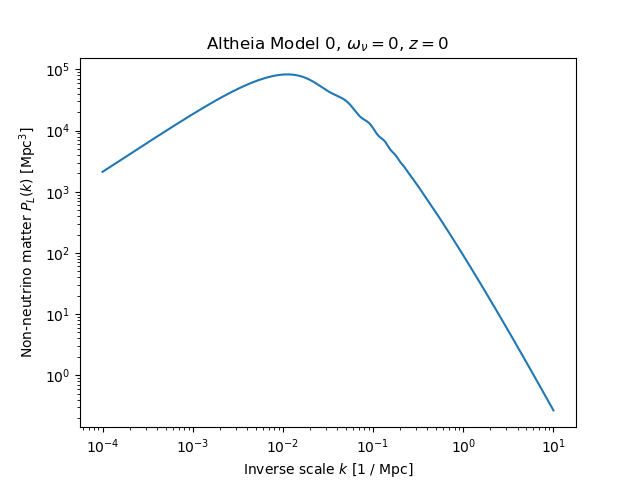
\includegraphics[scale=1.0]{intro/m0_Pk}
  \caption[Aletheia Model 0 Power Spectrum]{This is power spectrum was
  computed by CAMB for Aletheia model 0 without massive neutrinos.
  Table~\ref{tab: Aletheia_m0} defines this model in terms
  of the parameters essential to this work.}
  \label{fig: first_power_spectrum}
\end{figure}

\begin{table}[htb]
\centering
\begin{tabular}{l|l}
\hline
Parameter & Value \\ \hline
$\omega_b$ & 0.022445 \\
$\omega_c$ & 0.120567 \\
$n_s$ & 0.96 \\
$\sigma_{12}$ & 0.82476153 \\
$A_s$ & $2.1272 \cdot 10^{-9}$ \\ \hline
\end{tabular}
 \caption[Aletheia Model 0 Parameters]{This table describes
 figure~\ref{fig: first_power_spectrum} in terms of the parameters
 essential to this work. $A_s$ is truncated to five significant figures.
 Model 0 is a helpful benchmark model because it uses
 best-fit values from the Planck CMB measurements. Aletheia model 0 does not
 itself specify a physical density in neutrinos, but we will typically use
 $\omega_\nu = 0$. Unlike the rest of model 0, this setting is strongly 
 	discounted by our current cosmological observations.}
 \label{tab: Aletheia_m0}
\end{table}

The power spectrum for a standard Planck $\Lambda$CDM model is shown in
figure~\ref{fig: first_power_spectrum}. The turnover scale $k_\text{eq}$
(eq~\ref{eq: turnover}) marks
the transition between the radiation- and matter-dominated epochs, as
this mode enters the horizon (equation~\ref{eq: horizon}) at the time of
matter-radiation equality $t_\text{eq}$, such that:

\begin{equation}
\frac{\rho_\gamma}{a(t_\text{eq})^4}
=
\frac{\rho_m}{a(t_\text{eq})^3}
\end{equation} 

Figure~\ref{fig: first_power_spectrum} also shows the baryon acoustic
oscillation (BAO) as a set of shallow wiggles on inverse scales of roughly
$0.04 < k \, \text{Mpc} < 0.2$. The BAO is beyond the scope of this paper but,
briefly put, is the signature of a shock wave generated during the epoch of
radiation domination before baryons decoupled from photons. As baryons
collapsed into dark matter gravitational potential wells, the radiation
pressure eventually became high enough to reverse the collapse.

%s Everyone else uses h units. Why don't we?

Our power spectrum in
figure~\ref{fig: first_power_spectrum} does not use the customary $h$ units:
our $x$-axis uses units of Mpc$^{-1}$ rather than $h$ Mpc$^{-1}$ and our
$y$-axis uses units of Mpc$^3$ rather than Mpc$^3 \, h^{-3}$. 
Customary factors of $h$ (such as those that appeared in the $\Omega_i$
terms in section~\ref{sec: param_glossary}) are common in observational
cosmology.

The $h$-based units were introduced in the times when GRS redshift 
ranges contained very narrow redshift distributions. As mentioned in the
discussion on $\xi(r)$, the observed redshift of a galaxy can be transformed
into a comoving\footnote{the comoving coordinate system expands in the same
way as the Universe. Two objects without any relative velocity will always
remain at the same comoving separation from each other.} line-of-sight 
distance:

\begin{equation}
D_c (z)
=
\int_0^z \frac{c \, dz}{H_{100}}
\,
\left[
	\sum_i \omega_i (1 + z)^{3(1 + w_i)}
	+
	\omega_K (1 + z)^2
\right]^{-1/2}
\end{equation}

This requires the assumption of a \textit{fiducial cosmology}: a set of 
canonical values for cosmological parameters. However, at low
redshifts, this distance may be approximated as:

\begin{equation}
\label{eq: comov_dist_approx}
D_c(z) \approx \frac{c}{H_0} \, z
\end{equation}

Consequently, the use of $h$ units allowed early GRSs to present results
without committing to a fiducial cosmology. This
approximation loses its validity for later GRSs because of the larger redshift
values probed. Consequently, analyses of later GRSs needed to assume full 
fiducial cosmologies anyway, and the use of $h^{-1}$ Mpc units is no longer
advantageous. Nevertheless, they became convention and continue to be used 
\cbib{San20}.

% The following plots were generated with h_units_bad.ipynb
\begin{figure}[ht!]
    \begin{subfigure}{0.45 \textwidth}
    \centering
 		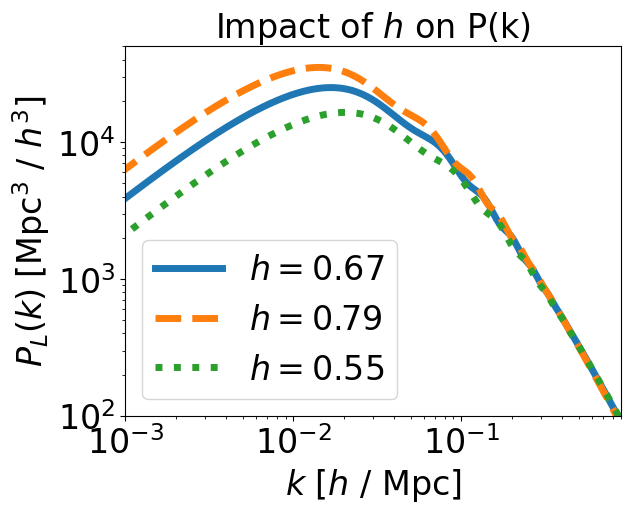
\includegraphics[width=\textwidth]{intro/h_impact_h_units}
 		\caption{Using $h$ units.}
 		\label{fig: h_units}
    \end{subfigure}
    \begin{subfigure}{0.45 \textwidth}
    \centering
 		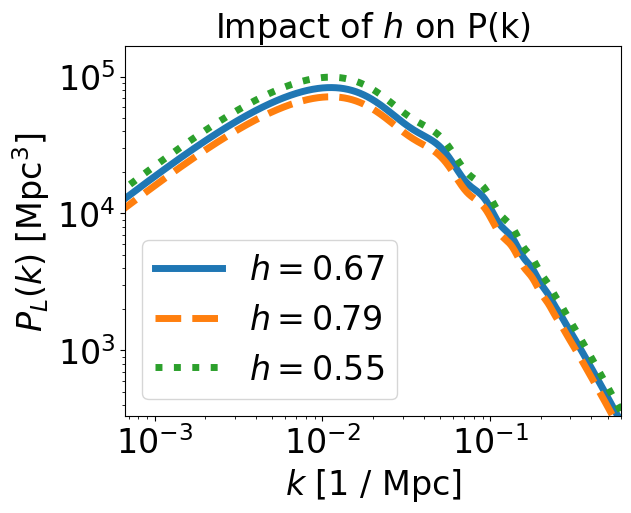
\includegraphics[width=\textwidth]{intro/h_impact_absolute_units}
 		\caption{Using absolute units.}
 		\label{fig: without_h_units}
    \end{subfigure}
        \centering
    \caption[Impact of $h$ on $P(k)$]
    		{Non-neutrino matter power spectra at $z=0$ for three different
    		models based on model zero (refer to table~\ref{tab: Aletheia_m0} 
    		for details) and varying only in the value of $h$. These two
    		panels
    		differ only in the units used. Observe that, in absolute units, we
    		can easily identify the impact of $h$ as a simple change in
    		amplitude. The use of $h$ units obscures this effect. This figure 
    		is an imitation of figure 1 from \citet{San20}.}
    \label{fig: h_unit_Pk}
\end{figure}

We illustrate in figure~\ref{fig: h_unit_Pk} one significant problem with the
use of $h$ units: varying $h$ changes not only the power 
spectrum, but also the axes used to represent the power spectrum. Comparison 
of power spectra from different 
models is hindered because the $x$ and $y$ axes correspond to different ranges
for each curve. If we use instead units of Mpc, then changes in $h$ affect
only the power spectrum, and we can much more readily appreciate its true
impact--that of an amplitude change.

%s Segue into the sigma parameters

There are several parameters that affect only the amplitude of the power 
spectrum. The physical density in curvature, $\omega_\nu$, is another example.
We call these parameters \textit{evolution parameters} to distinguish them
from \textit{shape parameters}, which affect the shape of the power
spectrum. To describe the amplitude of the power spectrum, we will use just 
one evolution parameter: $\sigma_{12}$ is defined as the linear-theory RMS 
mass variance in spheres of radius 12 Mpc:

\begin{equation}
\label{eq: sigma12}
\sigma_{12}
=
\sqrt{\left\langle \left(
	\frac{\delta M}{M} (12 \, \mathrm{Mpc})
\right)^2 \right\rangle}
\end{equation}

As with the $\omega_i$ parameters, there is a related parameter that
typically receives more attention: $\sigma_8$ is defined as

\begin{equation}
\sigma_8
=
\sqrt{\left\langle \left(
	\frac{\delta M}{M} (8 \, \mathrm{Mpc} \, h^{-1})
\right)^2 \right\rangle}
\end{equation}

Notice that this is \textit{not} the same as replacing 12 with 8 in
equation~\ref{eq: sigma12}! The subscript in $\sigma_8$ is misleading:
$\sigma_8$ is the linear-theory RMS mass variance in spheres of radius
$8 / h$ Mpc, not 8 Mpc. 

Our incomplete understanding of $h$ complicates the comparison of results
from different papers; if the quoted $h$ values differ even slightly, the same
symbol $\sigma_8$ will refer to different concepts--that is, mass variances on
different scales. Therefore, $\sigma_8$ comparisons will typically lead to
confusion, such as the $\sigma_8$ tension, which may be resolved by using
$\sigma_{12}$ instead.
For a fuller treatment of the advantages of $\sigma_{12}$, we
refer the reader to \citet{San20}.

For this work, the most relevant issue with $\sigma_8$ and the $\Omega_i$ 
parameters is their incompatibility with evolution mapping. The $\Omega_i$
parameters combine shape parameters like $\omega_b$ and $\omega_c$ with the
evolution parameter $h$, violating a distinction that we rely on in order
to simplify the parameter space. Although $\sigma_8$ behaves as an evolution
parameter for a fixed $h$, a varying $h$ will cause the meaning of $\sigma_8$
to change, and so we cannot rely on it to characterize the amplitude of the
power spectrum.


\section{Boltzmann Solvers and CAMB}
\label{sec: boltzmann_intro}

%s What kinds of equations do we need to solve?

The power spectrum can be predicted with great accuracy via linear 
approximations. However, the evolution equations are involved (running, for
example, over many different cosmological parameters) and can be
stiff, which calls for different approaches in different regimes. Furthermore,
its solutions are highly oscillatory and therefore susceptible to numerical
errors \cbib{Seljak}. Full solutions consist of many different steps, whose
descriptions fall outside of the scope of this work. We refer readers curious
about these equations to the history in the introduction of \citet{Seljak},
which cites papers important to their development. 

%s Equations are hard. Who can save us?

The so-called \textit{Boltzmann codes} have been 
developed in order to leverage modern computational power and automate the
solution of these equations of evolution. Typically, Boltzmann codes offer as
outputs CMB spectra and matter power spectra. The latter is the focus of this
work.

%s What can our savior do?

As input, Boltzmann codes accept a set of values for different 
cosmological parameters, many of which were defined in section~\ref{sec: 
param_glossary}. Boltzmann codes enable us to pick from wide ranges of 
accepted values for these parameters and to consider the power 
spectrum for almost any combination of these parameters. Of course, there are 
still limitations. For example, CAMB does not currently support negative 
redshifts (which, we will later see, becomes a problem), and the minimum 
allowed value of $H_0$ is 1 km s$^{-1}$ Mpc$^{-1}$, although slightly higher 
values have 
been observed to cause runtime errors in the presence of other extreme 
parameters. CLASS and CAMB claim to be accurate at the 0.1\% level
\cbib{Lesgourges}.

%s Pics? Not so fast. Let's pick one.

Before we proceed to concrete demonstrations, it will be expedient to settle
on a single Boltzmann solver. As of today, the two Boltzmann codes
CAMB\footnote{\url{https://github.com/cmbant/CAMB}} and
CLASS\footnote{\url{https://lesgourg.github.io/class_public/class.html}} offer
the largest suites of features and are also actively developed. CAMB and
CLASS were written in different languages (Fortran-90 and C, respectively)
but both come with Python wrappers. These codes have been shown to be in 
excellent agreement with each other (see \cbib{Lesgourges}), and their
differences consist primarily of different approaches in algorithms (including 
speedup tricks) and user interfaces and customization options.

As the researchers in our group have much more experience with CAMB, we 
elected to use CAMB as a starting point for our Python package
Cassandra-Linear. In principal, to maximize the generality of 
the results introduced in this 
work, we would demonstrate their compatibility with at least CLASS as well. In 
practice, since these codes agree so well, we prioritize other lines of 
inquiry
for this work. However, later, in section~\ref{sec: generate_emu_data}, we 
will concede an important, 
independent reason to consider use of CLASS, which becomes a promising route
for continuation of this work (see section~\ref{sec: future_work}).

%%%
\begin{comment}
\textcolor{green}{Furthermore, the CLASS documentation
is not nearly as strong as it is with CAMB, and we already encountered
extreme difficulty simply in recreating results already previously obtained
via CAMB!}
\end{comment}
%%%

%s Examples of great results from Boltzmann solvers

To connect this section with~\ref{sec: param_glossary}, we can visualize the
impact of each of this work's core parameters on the power spectrum. One
simple way to set this up for parameter $\Theta_i$ is to designate Aletheia 
model 0 as a middle ground and to create two copies of model 0, with each
copy tweaked to have an increased or decreased value of $\Theta_i$. This
approach works for every parameter except for $\omega_\nu$, where one of the
copy cosmologies describes the middle ground since the default value
$\omega_nu = 0$ is already at a hard boundary.

When feeding these cosmologies into CAMB, our Boltzmann solver of choice, we
obtain figures~\ref{fig: omega_b_dependence}, \ref{fig: omega_c_dependence}, 
\ref{fig: n_s_dependence}, \ref{fig: A_s_dependence}, and \ref{fig: 
omega_nu_dependence}. Keep in mind that the value ranges that we have applied
here are extremely broad and have nothing to do with state-of-the-art
confidence intervals on the parameters in our Unvirse. On the 
contrary, many of the values used for these plots may be completely 
discounted. The extreme values help us to clearly show the impact of each
parameter.

It should be
clear to the reader that each parameter has a special impact on the power
spectrum. None of these parameters is completely degenerate in the others,
although in the case of massless neutrinos $A_s$ and $\sigma_{12}$ are
completely degenerate, which is why we have not included an analogous plot for
$\sigma_{12}$ (the other reason being that CAMB does not accept $\sigma_{12}$
as an input--see section~\ref{sec: generate_emu_data}.

The remaining parameters $\sigma_{12}$ and $A_s$, as well as the quantities 
$z$ and $h$, all shift only the amplitude of the power spectrum. We show the 
amplitude shift associated with various $A_s$ values in figure~\ref{fig: 
A_s_dependence} and stress that the same plot only needs to be relabeled in 
order to illustrate the impact of $\sigma_{12}$, $z$, $h$, etc. 

\begin{figure}[ht!]
  \centering
  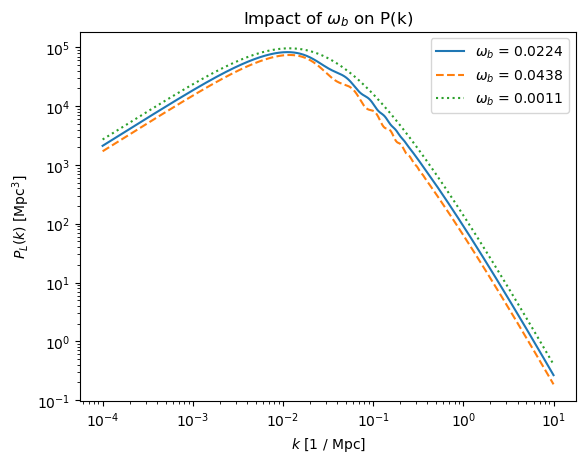
\includegraphics[scale=1.0]{intro/parameter_demos/ombh2_impact_on_Pk}
  \caption[Impact of $\omega_b$ on $P(k)$]{Impact of $\omega_b$. Increased
  	density in baryons corresponds to an increase in power on all scales.
  	However, this is not equivalent to a simple change in overall amplitude.
  	One counterexample is the shape of the BAO feature, which becomes more
  	pronounced for lower densities. A second counterexample is the location
  	of the turnover scale $k_s$, which is determined by the physical density
  	in baryons. However, this effect is subtle since the $x$-axis is
  	logarithmic and since even extreme values (relative to modern confidence
  	intervals) of $\omega_b$ will only slightly shift $k_s$. This shift
  	cannot be easily seen with the values used here.} 
  \label{fig: omega_b_dependence}
\end{figure}

\begin{figure}[ht!]
  \centering
  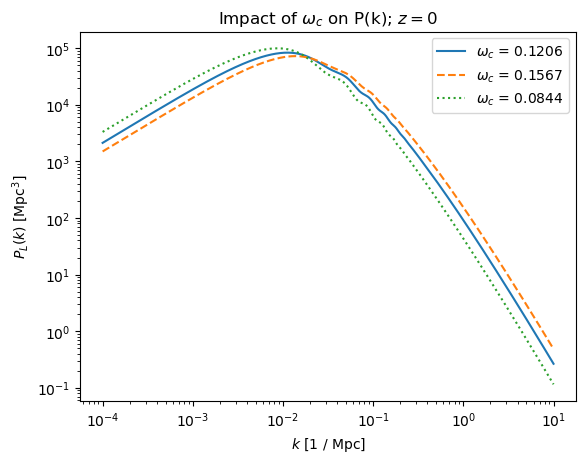
\includegraphics[scale=1.0]{intro/parameter_demos/omch2_impact_on_Pk}
  \caption[Impact of $\omega_c$ on $P(k)$]{Impact of $\omega_c$. Increased
  	density in CDM smooths out the BAO, similarly to the baryon case
  	(see figure~\ref{fig: omega_b_dependence}). More visibly, higher
  	densities shift power from larger to smaller scales due to gravitational 
  	collapse. Importantly, this behavior cannot be seen in the other
  	gravitationally interacting species, the baryons
  	(figure~\ref{fig: omega_b_dependence}). This is because, for all three
  	values used here for $\omega_c$ and for all three values used in
  	figure~\ref{fig: omega_b_dependence} for $\omega_b$,
  	$\omega_c > \omega_b$. This means that the baryon distribution will
  	largely be determined by the dynamics of CDM, rather than the
  	other way around. The dominant gravitationally-interacting species will
  	control the gravitational transfer of power from large to small scales.}
  \label{fig: omega_c_dependence}
\end{figure}

% If the gravitational collapse story were really true, why wouldn't that
% also apply to baryons? Maybe it's because b is so outnumbered by c

\begin{figure}[ht!]
  \centering
  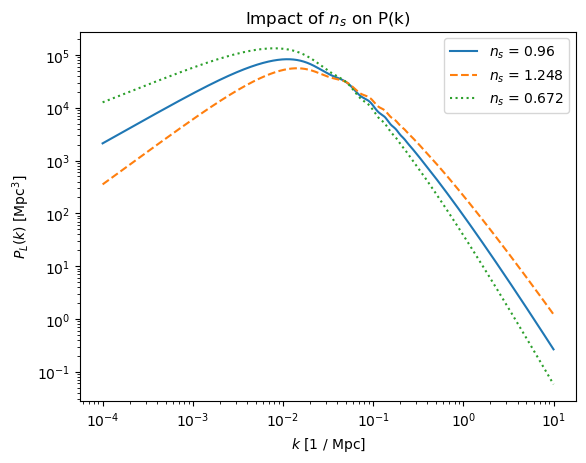
\includegraphics[scale=1.0]{intro/parameter_demos/n_s_impact_on_Pk}
  \caption[Impact of $n_s$ on $P(k)$]{Impact of $n_s$. The $n_s$ can be
  thought of as a kind of rotation of the power spectrum, although this
  is only coarse description. The differences shown here are
  adequately captured by equation~\ref{eq: n_s}.}
  \label{fig: n_s_dependence}
\end{figure}

\begin{figure}[ht!]
  \centering
  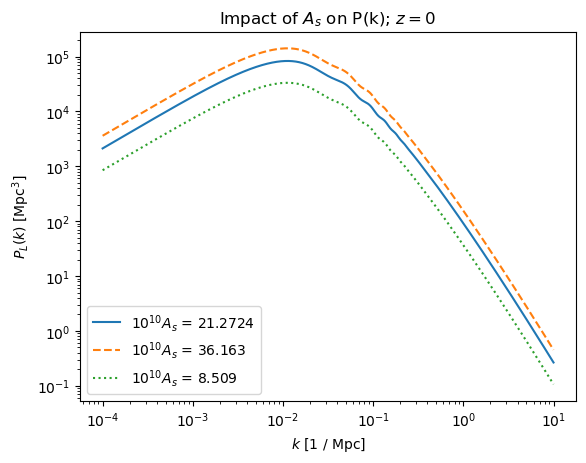
\includegraphics[scale=1.0]{intro/parameter_demos/A_s_impact_on_Pk}
  \caption[Impact of $A_s$ on $P(k)$]{Impact of $A_s$. Differences produce
  	only a change in the overall amplitude of the power spectrum. We stress
  	that this simple description applies only in the case of massless
  	neutrinos. The more subtle impact of $A_s$ will be demonstrated in
  	chapter~\ref{chap: A_s}. In the massless case, $A_s$ is completely
  	degenerate with $h$ (see figure~\ref{fig: without_h_units}) and with
  	$\sigma_{12}$ (not shown). This degeneracy is central to evolution
  	mapping, which will be discussed in section~\ref{sec: ev_mapping_intro}.}
  \label{fig: A_s_dependence}
\end{figure}

\begin{figure}[ht!]
  \centering
  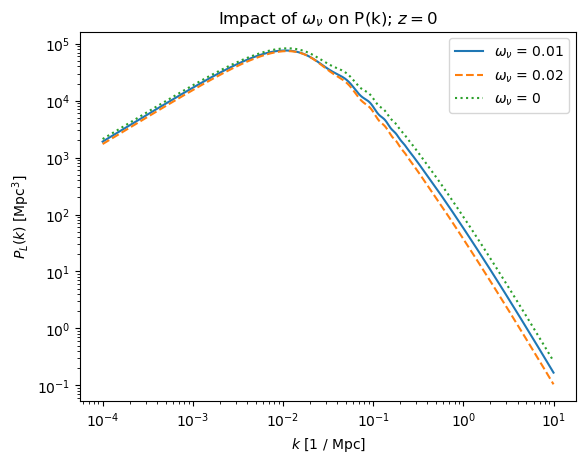
\includegraphics[scale=1.0]{intro/parameter_demos/omnuh2_impact_on_Pk}
  \caption[Impact of $\omega_\nu$ on $P(k)$]{Impact of $\omega_\nu$ for the
  	fixed redshift $z=0$. Massive neutrinos suppress structure formation in
  	a manner highly reminiscent of radiation. This similarity arises from the
  	combination of neutrinos' large velocities with the weakness of their 
  	interaction with other particles.
  	For the other primary parameters of this work,
  	the impact on power spectrum is independent of the value of $z$. This is
  	not the case with massive neutrinos
  	(see figure~\ref{fig: neutrinos_and_redshift}), which we will discuss in
  	section~\ref{sec: neutrino_problem}.}
  \label{fig: omega_nu_dependence}
\end{figure}

%s Segue into the next section

Since many of these parameters have fairly unique impacts on the power 
spectrum, we can imagine building a collection of power spectra labeled by
their parameter configurations and then comparing our real-world observations 
to them. We can ask to which of these theoretical power spectra our 
observations most closely agree. This question is quantitatively answered by 
parameter inference in the form of a Monte Carlo Markov Chain (MCMC) analysis, whose basic idea will be discussed in the next section.

%%% We're sinking this section! It's not relevant enough and I don't know 
%%% enough.
\begin{comment}

\section{Monte Carlo Markov Chains}

%Bayes' theorem states that

%\begin{equation}
%P(\bm{\pi} | \bm{d}) 
%\end{equation}

%We can assign a probability $P(\bm{\pi} | d$

This can be a very brief section, but I want to discuss a little bit of how most modern parameter inference works because it motivates the need for extremely fast power spectrum computation. It provides a sort of conceptual bridge between our ``pure'' goal (quantifying the cosmos) and the nitty-gritty bulk of the paper (optimizing emulator performance).

Metropolis-Hastings algorithm.

We don't know what the true probability distribution of power spectra is. In order to build this distribution with simulation results, we simply draw from the distribution. \textcolor{orange}{Refer to ``Data to Insights'' lecture notes in order to tighten this description.}

\end{comment}
%%%

\section{Evolution Mapping}
\label{sec: ev_mapping_intro}

\citet{San21} proposes to divide up the full set of cosmological
parameters into the two categories introduced in section~\ref{sec: Pk_intro}: 
shape parameters $\Theta_s$ and evolution parameters $\Theta_e$.
Shape parameters affect the shape of the power spectrum. Examples include
$\omega_b$, $\omega_c$, and $n_s$.
Evolution parameters affect only its amplitude. They are so called because
their impact on the linear-theory power spectrum is 
indistinguishable from a time evolution of the power 
spectrum. This means that varying the redshift at which we evaluate the power
spectrum will affect only its amplitude. $h$, $\omega_k$ and
$\omega_\text{DE}$ are examples of evolution parameters. 

We adapt equation 13 from \citet{San21} to write:

\begin{equation}
\label{eq: evMapping_pSpectrum}
    P_L (k | z, \Theta_s, \Theta_e)
    =
    P_L (k | \Theta_s, \sigma_{12} \left( z, \Theta_s, \Theta_e \right))
\end{equation}

which we call the \textit{evolution mapping relation} for the power
spectrum.\footnote{As mentioned before, varying $z$ has the effect of varying 
an evolution parameter, so it appears on the RHS only as an argument 
to the $\sigma_{12}$ ``function.'' We write it separately from
$\Theta_e$ to
emphasize that $z$ does not describe a property of the Universe, but is
simply used as a proxy here for \textcolor{red}{conformal?} time
\textcolor{red}{elapsed since the Big Bang? (but we can only observe up to
$z = 1100$...)}.} 
We stress that the evolution mapping relation does not hold when $P_L$ is
expressed in $h$ units.

%s In action: relabel some power spectra

The evolution mapping relation tells us that any two cosmologies with 
identical shape
parameters will yield identical power spectra as long we match the value of
$\sigma_{12}$. This matching can be accomplished merely by varying the 
redshift at which the power spectrum is evaluated.
Figure~\ref{fig: ev_mapping_demo} shows the results of this technique applied
to seven different cosmologies sharing shape parameters and differing only
in evolution parameters.

\begin{figure}[ht!]
  \centering
  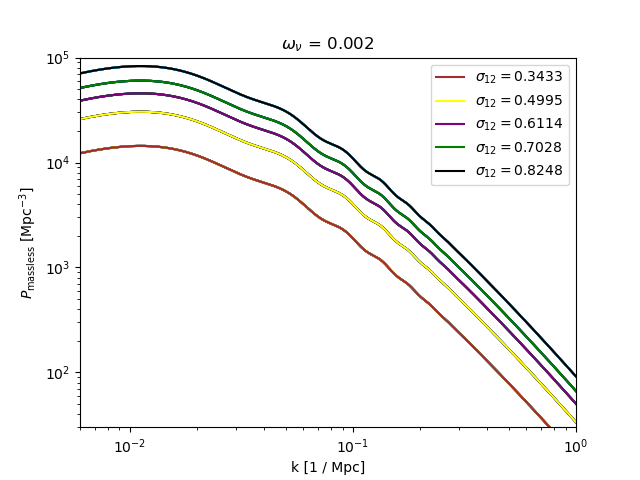
\includegraphics[scale=1.0]{intro/san21f2}
  \cprotect\caption[Demonstration of evolution mapping]{Power spectra matched
  	in $\sigma_{12}$ via evaluation at different redshifts. For each value of
  	$\sigma_{12}$
  	shown here, eight Aletheia models were plotted in different
  	colors. Each set of lines is tightly distributed and thereby demonstrates 
  	the excellent agreement of power spectra from $\sigma_{12}$-matched
  	cosmologies that agree in their shape parameters. This figure was
  	inspired by figure 2 from \citet{San21}. Aletheia model 0 was related in
  	table~\ref{tab: Aletheia_m0}. For details on the rest of the Aletheia
  	models, please refer to the file
  	\verb|cosmologies.dat|\footnote{\url{https://github.com/3276908917/Master/blob/main/cassL/cosmologies.dat}}
  	in the Cassandra-Linear GitHub repository.}
  \label{fig: ev_mapping_demo}
\end{figure}

%s Now conclude with the significance

Evolution mapping is essential to this work because it greatly simplifies the 
parameter space over which we train our emulator. We can express the impact of
all evolution parameters through their impact on $\sigma_{12}$. Consequently, 
we need only train the emulator over the shape parameters and $\sigma_{12}$.
Simplifying the parameter space will
result in increased accuracy for our emulator because our training samples
will be efficiently distributed throughout the parameter space. By contrast,
if we explicitly trained over additional evolution parameters, the same set of
training samples would much less densely cover the parameter space.

\textcolor{red}{A segue into neutrinos would be possible here, but it
wouldn't look too good since the neutrino section comes at the end. Should I
put the neutrino section right after this one?}

% To-do:

% Make the plot where the different models overlap through sigma-matching

\section{Emulation}
\label{sec: emulation_intro}

Boltzmann codes typically take on the order of three seconds to evaluate the
linear matter power spectrum for a given cosmological configuration. In a
modern Monte Carlo Markov Chain analysis, tens of thousands of such
configurations will need to be evaluated. Therefore, power
spectra evaluation becomes a bottleneck of the analysis.

This motivates the use of emulators, which rely on multi-dimensional 
interpolation instead of the equations of evolution. Emulators are trained 
over large numbers of power spectra either computed
by a Boltzmann solver or from an N-body simulation. Power spectra emulation 
has been shown to achieve excellent accuracy with computation times shorter
by several orders of magnitude.\footnote{Of course, the accuracy of a
well-constructed emulator will ultimately still be limited by the accuracy of 
the input power spectra. Recall in the case of CAMB that this is 0.1\%
\cbib{Seljak}.}

Emulators apply different machine
learning approaches in order to transform between cosmological
configurations and power spectra. The two most common choices are neural 
networks (NNs), which optimize the weights and biases on a set of connected 
nodes, and Gaussian process regressions (GPRs), which apply Bayes' theorem to  
iteratively tighten the variance of a distribution of random functions.

Emulators interpolate across a high-dimensional parameter space. This presents
a fundamental limitation: emulators must be built with the same parameter
space over which end users require for their analyses. If additional
parameters or wider priors are needed, then new emulators need to be trained.
Yet there is a large number of different cosmological parameters discussed in 
the modern literature. Emulator flexibility and generality is desirable, but 
comes at the price of a significantly more sample-expensive training phase in
order to maintain accuracy levels.

However, due to the
generality-accuracy tradeoff, currently available emulators tend to sample
only sample a few cosmological parameters and over restrictive ranges
\cbib{San21}. \textcolor{red}{This comment only applied to the emulators
trained over N-body simulations, right? So it would probably be inappropriate
to mention it in this paper, since we are emulating over Boltzmann solver
spectra}.
% Also part of this cut paragraph:
\begin{comment}
	``Due to the high computational cost of the required
	simulations, [...] current emulators leave out parameters such as the
	curvature of the Universe or dynamic energy models beyond the standard CPL
	parametrization'' (\cbib{San21}).
\end{comment}

The effectiveness of emulation has given rise to considerable popularity, and
several emulators of linear and nonlinear power spectra have been put 
forth in the literature.\footnote{Linear and nonlinear power spectra have 
different
applications. Linear power spectra can be used to predict $P_\text{NL}(k)$, 
such as in perturbation theory approaches. Furthermore, most non-linear 
emulators actually predict the ratio of the non-linear power spectrum to its 
linear counterpart, so $P_\text{L}(k)$ is still necessary to evaluate
$P_\text{NL}(k)$ (A. G. S\'{a}nchez, private communication, 2022).}
\verb|baccoemu| includes both nonlinear and linear power spectrum emulators 
based on NNs. The quoted accuracies in the linear case are
0.2\% for redshifts $z \lesssim 3$ and
0.5\% for redshifts $z \lesssim 9$. This emulator is trained over 216000
\verb|CLASS|
models in 600 $k$-bins $10^{-4} \leq k$ [$h$ Mpc$^{-1}$] $\leq 50$ and 
includes massive neutrinos \cbib{Arico}. \verb|CosmoPower| also uses an NN
to emulate both linear and nonlinear power spectra. It was trained over
180,000 spectra in 420 $k$-bins over the ranges
$10^{-5} \leq k $ Mpc$^{-1} \leq 10$ and 
$0 \leq z \leq 5$. The authors have verified
its accuracy on a full inference pipeline, demonstrating that the results
are in excellent agreement regardless of the choice between \verb|CAMB| and
\verb|CLASS| for the calculation of the training spectra. In the linear case,
\citet{Mancini} quote errors of less than 0.1\%. 

\verb|COMET| is of particular interest to this work because it has already
successfully demonstrated the application of evolution mapping to the task of
linear power spectrum emulation. \verb|COMET| uses GPR, although the 
development team
has recently decided to switch to an NN \cbib{Eggemeier}.

\textcolor{orange}{I need material on the accuracy and ranges over which
COMET can operate.}

% Other things we could talk about: make more explicit that we are using a
% large # Boltzmann / N-body power spectra in order to train the emulator in
% the first place. This of course means that the accuracy will eventually be
% limited by the accuracy of the input spectra...

% This section really is short. Am I forgetting to talk about anything?

\section{Gaussian Process Regression}
\label{sec: gpr_intro}

In this work, we apply a GPR to emulate power spectra. A Gaussian Process 
(GP) is a Gaussian distribution over random functions,\footnote{The functions
themselves are deterministic.} which can be interpreted
as the infinite-dimensional generalization of the multivariate normal
distribution. The inference of continuous values with a GP prior
is known as Gaussian process regression, or Kriging. GPR is a
powerful non-linear multivariate interpolation tool because in addition to
allowing conventional predictions, GPR can also give us an uncertainty on the
prediction, which is not typically obtained when training an NN.

\textcolor{red}{Should I put some equations here, to outline the basics?
For example, I could refer to
\url{https://gaussianprocess.org/gpml/chapters/RW.pdf} as the COMET paper
does.}

NNs represent the most common approach in the literature. We elect to use a
GPR for this work for several reasons. Most importantly, we find it to be
a considerably simpler approach, more accessible to novices.
NNs invariably require much more complicated setup and tuning in the precise 
architecture and hyperparameter values (nodes per layer, learning rate, etc.) 
By contrast, as we explain in section~\ref{sec: train_emu}, a Gaussian
process regression is highly straightforward to set up and modify.

Furthermore, NNs generally need much larger sample sizes to reach comparable 
levels of accuracy. Due to various alterations in the Cassandra-Linear code 
over its development, several regenerations of the various emulator data sets 
were necessary. This practical constraint motivated the use of a GP for our
emulator. Please refer to the section~\ref{sec: future_work} for a
continuation of the comparison between NNs and GPRs for emulation tasks.

\textcolor{orange}{Are there other prediction approaches besides GPs and NNs? 
If so, I need to further justify WHY we’re using GPs.
GPs work best when there are few samples and a lot of 
parameters, right? But why is that so? What is the math behind that?}


\section{Sampling Approach: Latin Hypercube}
\label{sec: lhc_theory}

%%% It's just not relevant, we're only predicting later, and we've already
%%% demonstrated that GPR is faster than Boltzmann.
\begin{comment}
The computational complexity of inference and likelihood evaluation within GPR 
is cubic in the number of points \cbib{Barber}.
This makes GP regression an excellent companion to
Latin hypercube sampling (LHS), which makes highly efficient use of a limited 
number of samples.
\end{comment}
%%%

We will need to build several data sets in order to train and test our
emulator. Now that we have decided on the parameters whose effects we would
like to emulate, we need to sample these parameters in order to build
individual cosmologies. We will use Latin hypercube sampling to sample 
the space of cosmological configurations.

A unit Latin hypercube sample (LHS) is primarily characterized by its 
dimension $d$ and number of 
samples $N_s$. $d$ separate intervals, all running from zero to unity, are
each split into $N_s$ subintervals. Then, each subinterval is sampled
exactly once. By contrast, simple random sampling (SRS) may sample any 
particular subinterval any number of times, including not at all. SRS
can require vast numbers of samples before all regions of the space are
represented. For a pictorial representation of SRS versus Latin hypercube
sampling, see figure~\ref{fig: sample_comparison}.

% The following plots were generated with h_units_bad.ipynb
\begin{figure}[ht!]
    \begin{subfigure}{0.32 \textwidth}
    \centering
 		\includesvg[width=\textwidth]{intro/lhs/random}
 		\caption{A random sample. Some subintervals are sampled repeatedly.}
 		\label{fig: random_sample}
    \end{subfigure}
    \begin{subfigure}{0.32 \textwidth}
    \centering
 		\includesvg[width=\textwidth]{intro/lhs/bad_LHS}
 		\caption{An LHS with a low minimum separation between points.}
 		\label{fig: poor_lhs}
    \end{subfigure}
    \begin{subfigure}{0.32 \textwidth}
    \centering
 		\includesvg[width=\textwidth]{intro/lhs/better_LHS}
 		\caption{A different LHS with a higher minimum separation between
 			points.}
 		\label{fig: better_lhs}
    \end{subfigure}
    \centering
    \caption[Comparison of SRS and Latin hypercube sampling.]{Comparison of an 
    example
    	random sample with two examples of LHSs. Unlike random sampling,
    	Latin hypercube sampling guarantees that every subinterval will be 
    	sampled. However, if
    	the minimum separation is low enough, there will still be large
    	undersampled regions.}
    \label{fig: sample_comparison}
\end{figure}

Latin hypercube sampling does not always improve significantly over SRS. It is 
convenient to
assess the quality of an LHS according to the minimum separation $s^*$ 
between any two sample points in the LHS. A high $s^*$ indicates that 
the sample space is evenly covered. To visually appreciate the difference 
between LHSs of different $s^*$ values, see again
figure~\ref{fig: sample_comparison}.

For each value of $d$ and $N_s$, there is a theoretical maximum value of
$s^*$:

\begin{equation}
\label{eq: best_lhs_sep}
s^*_\text{best} = \left( \frac{1}{N_s} \right)^{1 / d}
\end{equation}

For example, for a six-parameter emulator trained over 5000 samples, the best
possible LHS sample would have $s^* \approx 0.2418$.
\textcolor{orange}{Talk about how you got this equation?}

Once we have a unit LHS, we can rescale each coordinate according to a 
different parameter's prior to map the LHS into our parameter space. The
choice of priors will be discussed in the conceptual outline of our
emulator (see section~\ref{sec: default_priors}). Similarly,
although the unit LHS entails linear sampling of the [0, 1] interval, it is 
straightforward to transform these samples into a different distribution
the interpretation stage (section~\ref{sec: lhc_flow_chart}).

\section{Neutrinos and Their Cosmological Impact}
\label{sec: neutrino_problem}

As mentioned in section~\ref{sec: emulation_intro}, COMET has already 
successfully demonstrated the application of evolution mapping to emulation. 
The focus of this work is to extend evolution mapping (EvM) to account for 
massive neutrinos. Due to uncertainty about how to handle $\omega_\nu$ within 
the evolution mapping framework, COMET fixes this parameter at zero.

At this point, we add that we are focusing on the power
spectrum of \textit{non-neutrino} matter.\footnote{\textcolor{red}{Andrea 
added the following comment: ``We should 
justify this assumption. It is standard practice to assume that the galaxy 
density field is determined only by the underlying cdm+b density field, 
without taking into consideration the cold neutrino component (which also 
behaves as matter).'' Do you have recommendations for sources I can consult in
order to add this information to this paragraph?}} Several currently-available 
emulators, such as \verb|baccoemu| and \verb|CosmoPower|, are able to handle 
massive neutrinos because they do not use evolution mapping.

Evolution mapping relies on a clear separability in parameters which massive 
neutrinos do not cleanly follow. Specifically, unlike other shape parameters, 
the impact of $\omega_\nu$ on the power spectrum is not constant in redshift
(see figure~\ref{fig: neutrinos_and_redshift}.
Due to the extremely low mass per particle, and the lack of charge, neutrinos
interact only extremely weakly with baryonic matter. Neutrinos behave like a 
relativistic species in the extremely hot and energetic early Universe.
During this period, neutrinos suppress structure growth on small scales by
free-streaming out of overdensities \cbib{Kiakotou}. As the Universe expands 
and cools down, neutrinos gradually behave like increasingly cold dark matter,
which promotes structure growth.

\begin{figure}[ht!]
  \centering
  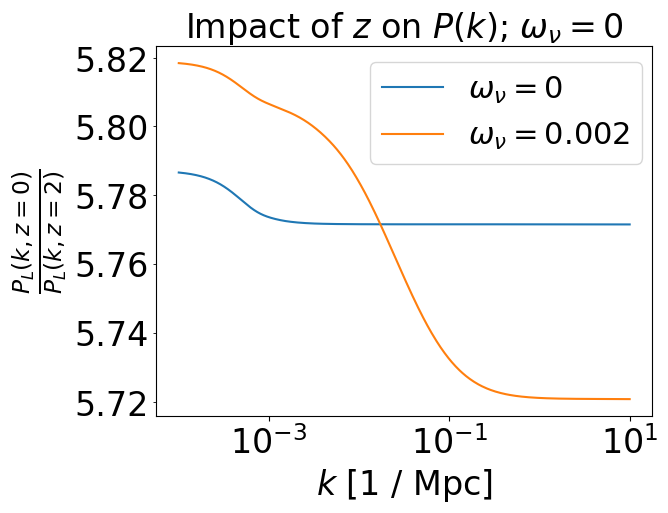
\includegraphics[scale=0.5]{intro/redshift_dependence_problem}
  \caption[Redshift Dependence of Neutrino Impact]{Ratio of the power spectrum
  	at $z = 0$ and $z = 2$. Observe that when the cosmology features massive
  	neutrinos, the ratio is subject to much higher dynamic range. Therefore,
  	in massive neutrino cosmologies, the redshift no longer effects a
  	mere overall amplitude shift.}
  \label{fig: neutrinos_and_redshift}
\end{figure}

Whenever massive neutrinos are present, the growth factor becomes scale-
dependent, which disrupts the application of evolution mapping. There have
been several proposals for isolating and approximating the impact of 
neutrinos. For example, \citet{Kiakotou} includes a popular formula for
linear-theory suppression of matter fluctuations:

\begin{equation}
\Delta P(k) / P(k) \approx -8 f_\nu
\end{equation}

which is unfortunately valid only on very small scales $k > 0.8 h$ / Mpc.

It has also been proposed to treat the neutrinos as a small correction factor
to the results from an analogous cosmology with the same $\omega_m$ but with
$\omega_\nu = 0$. This limits the applicability of our emulator to
cosmologies with very small $\omega_\nu$, where we can treat the effect of
massive neutrinos as a perturbation on our massless-neutrino spectra. We adapt 
the evolution mapping relation as follows:

\begin{equation}
\label{eq: evMapping_modded}
    P_L (k | z, \Theta_s, \Theta_e)
    =
    P_L (k | \Theta_s,
    		\tilde{\sigma}_{12} \left( z, \Theta_s, \Theta_e \right))
\end{equation}

%s what is a MEMNeC?

and then treat the physical density in neutrinos as a shape parameter.
We define $\tilde{\sigma}_{12}$ as the $\sigma_{12}$ of the corresponding 
matter-equivalent massless-neutrino cosmology (MEMNeC). The MEMNeC is
defined such that $\tilde{\omega}_c = \omega_c + \omega_\nu$ and
$\tilde{\omega}_\nu = 0$.

The goal of this work is to improve on this solution after exploring the 
impact 
of massive neutrinos in greater depth. In the next chapter, we will carefully 
explain our CAMB setup, which will allow us to test possible improvements.